\documentclass[aspectratio=169]{beamer}
\usepackage[utf8]{inputenc}               % codificacao de caracteres
\usepackage[T1]{fontenc}                  % codificacao de fontes
\usepackage[english,brazilian]{babel}     % idioma
\usetheme{Madrid}                         % tema
% \usecolortheme{orchid}                  % cores
\usefonttheme[onlymath]{serif}            % fonte modo matematico
% \usepackage[authoryear,round,longnamesfirst]{natbib}
\usepackage{graphicx}
% Pacote para escrever algorítmos no Latex
\usepackage[ruled,vlined]{algorithm2e}

% Titulo
\title[\sc{Três Ensaios em Comportamentos dos Preços}]{Três Ensaios em Comportamento dos Preços na Economia Brasileira}
\author{Hudson Chaves Costa}
\institute{PPGE - UFRGS} 
\date{\today}


\usepackage{Sweave}
\begin{document}
\Sconcordance{concordance:apresentacao.tex:apresentacao.Rnw:%
1 24 1 1 0 444 1}



\begin{frame}
  \titlepage
Orientador: Prof. Dr. Sabino Porto da Silva Júnior
\end{frame}

\begin{frame}[plain]\frametitle{Sumário}
\small\tableofcontents
\end{frame}

\section{Ensaio 1}
  
\begin{frame}\frametitle{}
	\begin{center}
	{\Huge Ensaio 1}
	\end{center}
\end{frame}

\subsection{Introdução/Motivação}

\begin{frame}\frametitle{Introdução/Motivação}
  \begin{itemize}
  \item Firmas individuais não ajustam seus preços em contrapartida de choques relevantes na economia:
    \begin{itemize}
    \item Hipótese em modelagem macroeconômica;
    \end{itemize}
  \item Comportamento microeconômicos de determinação de preços adotado pelos agentes:
    \begin{itemize}
    \item Tempo-Dependente;
    \item Estado-Dependente.
    \end{itemize}
  \item Bancos Centrais têm usado a política de metas de inflação:
    \begin{itemize}
    \item Meta definida em termos de um índice de preços agregado;
    \item Rigidez x Flexibilidade nos preços.
    \end{itemize}
  \item A partir disso, foi natural o surgimento de pesquisas com o objetivo de diferir a análise empírica da rigidez nominal dos preços baseada em dados agregados da avaliação do comportamento dos preços por meio de microfundamentos.
  \end{itemize}
\end{frame}

\subsubsection{Justificativa}

\begin{frame}\frametitle{Introdução/Motivação}
\textbf{Justificativa}
\begin{itemize}
% \item Em particular, \citet{bils2004some,nakamura2008five,klenow2008state,dhyne2006price,gouvea2007nominal,matos2009comportamento,lopes2008rigidez,bunn2012examining}.
\item A dinâmica do comportamento dos preços individuais proporciona vários desdobramentos que são bastantes debatidos na literatura dado o impacto que podem causar;
  \begin{itemize}
  \item A sua não compreensão levou a distintas abordagens para a análise da velocidade e intensidade de transmissão da política monetária
  \end{itemize}
\item A falta de estudos que gerassem empiricamente um diagnóstico da definição e grau de rigidez de preços individuais;
\item Limitação de acesso a base de dados
\end{itemize}
\end{frame}

\subsubsection{Objetivos}

\begin{frame}\frametitle{Introdução/Motivação}
\textbf{Objetivos}
\begin{itemize}
\item Avaliar empiricamente a rigidez nominal dos preços na economia brasileira por meio de dados coletados da \emph{web}
\item Propor um índice de inflação oriundo da mesma fonte de dados;
\item Questinamentos:
  \begin{itemize}
  \item É possível utilizar os dados coletados da internet como \emph{proxy} para a inflação divulgada pelos órgãos públicos?
  \item Quão frequentemente os preços se alteram?
  \item Existe heterogeneidade da rigidez nominal entre setores?
  \item A probabilidade de mudança dos preços pode variar ao longo da duração dos preços?
  \item Quais são as variáveis condicionantes para o risco de alteração nos preços?
  \end{itemize}
\end{itemize}
\end{frame}

\subsection{Referencial Bibliográfico}

\begin{frame}\frametitle{Referencial Bibliográfico}
  \begin{itemize}[<+->]
  \item Modelos de Precificação
    \begin{itemize}
      \item Contratos de Calvo/Taylor
      \item Custo de Menu
      \item Informação Rígida
      \item Ira do Cliente
    \end{itemize}
  \item Preços Rígidos e Preços Flexíveis
  \item Modelos Tempo-Dependente e Estado-Dependente
  \item Estudos Empíricos
  \end{itemize}
\end{frame}

\begin{frame}\frametitle{Referencial Bibliográfico - Modelos de Precificação}
  \textbf{Contratos de Calvo/Taylor}
  \begin{itemize}
  \item No modelo de Calvo (1983) a probabilidade de um preço mudar é constante:
    \begin{itemize}
      \item Independe da última vez que uma firma mudou seu preço;
      \item Função risco constante.
    \end{itemize}
  \item Taylor (1980) define que os preços nominais são fixos por um certo número de períodos:
    \begin{itemize}
      \item Os preços são fixos por N períodos;
      \item Taxa de risco é zero para todas as durações exceto N.
    \end{itemize}
  \item Generalização dos modelos de Taylor e Calvo:
    \begin{itemize}
      \item Em Taylor, existem muitos setores com diferentes tamanhos de preços e dentro de cada setor há um processo de Taylor simples;
      \item Em Calvo, a estratégia de definição dos preços considera múltiplos setores.
    \end{itemize}
  \end{itemize}
\end{frame}

\begin{frame}\frametitle{Referencial Bibliográfico - Modelos de Precificação}
  \textbf{Custo de Menu}
  \begin{itemize}
  \item Assume que a mudança no preço é custosa e isto impede que as firmas alterem seus preços continuamente;
  \item Os modelos usualmente são resolvidos usando métodos numéricos e assim, não há expressão analítica para a taxa de risco.
  \end{itemize}
  \textbf{Ira do Cliente}
  \begin{itemize}
  \item Modelo de Rotemberg (2005) salienta que os clientes sempre analisam as decisões de precificação das firmas;
  \item Percepção de justiça;
  \item Firmas podem abandonar alterações nos preços para evitar a ira do cliente;
  \item Em rápido crescimento da inflação os clietnes aceitam os ajustes dos preços;
  \item Empresas podem alterar seus preços dentro de um calendário de forma que os clientes desenvolvam suas crenças.
  \end{itemize}
\end{frame}

\begin{frame}\frametitle{Referencial Bibliográfico - Modelos de Precificação}
  \textbf{Informação Rígida}
  \begin{itemize}
  \item Firmas sofrem com o custo de coletar informações sobre as condições econômicas e concorrentes;
  \item Em cada período, a partir de novas informações, define-se um novo padrão de preços ótimos;
  \item Todas as firmas mudam seus preços em todo o tempo em modelos de rigidez de informação;
  \item Contudo, é contraditório nas evidências empíricas baseadas em dados individuais;
  \item Estudos combinaram este modelo com custo de menu (Klenov e Willis, 2007;II e Edward, 2010)
  \item \textbf{Solução:} Pagar custos ou aprender com as ações das outras empresas.
  \end{itemize}
\end{frame}

\begin{frame}\frametitle{Referencial Bibliográfico - Preços Rígidos e Preços Flexíveis}
  \begin{itemize}
  \item A alternativa aos modelos de preços rígidos é o modelo de \textbf{Lucas (1972)} onde os preços são flexíveis e a imperfeição nominal é informacional;
    \begin{itemize}
    \item Produtor observa uma mudança no preço do seu produto e não sabe distinguir se isso é resultado de alterações no preço relativo ou nível agregado de preços;
    \item A partir de uma expansão monetária não-observada, o melhor que cada produtor pode fazer é admitir que uma parte do aumento da demanda por seu produto reflete um choque de preços relativos;
    \item \textbf{Consequência:} Expansão monetária tem efeitos reais e não apenas nominais sobre os preços.
    \end{itemize}
  \end{itemize}
\end{frame}

\begin{frame}\frametitle{Referencial Bibliográfico - Preços Rígidos e Preços Flexíveis}
  \begin{itemize}
  \item A vertente \textbf{novo-keynesiana} estabelece a hipótese de existência de rigidez nominal tanto nos preços quanto nos salários;
  \item Essas variáveis nominais têm dificultade de ajuste e provocam impactos reais sobre o produto;
  \item \textbf{Consequência:} Expansão monetária pode causar diferentes impactos sobre cada preço da economia dependendo do grau de rigidez nominal de cada bem;
  \item \textbf{Consequência:} Se a rigidez for diversificada, resultará em alterações nos preços relativos provocando impactos reais
  \end{itemize}
\end{frame}

\begin{frame}\frametitle{Referencial Bibliográfico - Modelos Tempo-Dependente e Estado-Dependente}
\textbf{Tempo-Dependente}
  \begin{itemize}
  \item A probabilidade dos preços mudarem depende apenas do período pelo qual o preço está fixo;
  \item Função risco tem um forma constante em relação à duração dos preços
  \item Calvo (1983) assume uma função risco plana:
    \begin{itemize}
    \item Oportunidade de alterar os preços com uma probabilidade constante em cada período;
    \item Curva de Phillips Novo-Keynesiana é derivada do modelo de Calvo com competição monopolística.
    \end{itemize}
  \item Taylor (1980) tem uma função risco constante:
    \begin{itemize}
    \item Preços mudam no começo do contrato e não se alterarm dentro do período de durabilidade;
    \item Taxa de risco toma o valor da unidade no começo do contrato e 0, por conseguinte. 
    \end{itemize}
  \end{itemize}
\end{frame}

\begin{frame}\frametitle{Referencial Bibliográfico - Modelos Tempo-Dependente e Estado-Dependente}
\textbf{Estado-Dependente}
  \begin{itemize}
  \item Custo de Menu de Barro (1972) e Sheshinski e Weiss (1977);
  \item Tendem a ter maior fundamentação microeconômica;
  \item Probabilidade condicional do preço alterar depende das variáveis de estado, preços relativos e taxas de inflação;
  \item Função risco pode mudar sua forma em resposta à choques reais ou monetários em transição;
    \begin{itemize}
    \item Forma constante em \emph{steady state}
    \end{itemize}
  \end{itemize}
\end{frame}

\begin{frame}\frametitle{Referencial Bibliográfico - Estudos Empíricos}
  \begin{itemize}
  \item Trabalhos utilizando microdados para analisar a rigidez nominal nos preços;
  \item Viabilidade de avaliação da rigidez em vários níveis (setores, cidades, cesta de consumo, ...);
  \item \textbf{Bils e Kenow (2004)}:
    \begin{itemize}
    \item Alterações nos preços mensais de 350 produtos e serviços que representavam em torno de 70\% da cesta de consumo do CPI no período de 1995 a 1997 nos EUA;
    \item \textbf{Conclusão:} Os preços se alteravam tipicamente em torno de uma vez por ano
    \end{itemize}
  \end{itemize}
\end{frame}

\begin{frame}\frametitle{Referencial Bibliográfico - Estudos Empíricos}
  \begin{itemize}
  \item \textbf{Nakamura e Steinsson (2008)}:
    \begin{itemize}
    \item Avaliaram os preços mensais de 270 produtos que representavam 70\% da cesta de consumo do CPI no período de 1998 a 2005 para os EUA;
    \item \textbf{Conclusões:} 
      \begin{itemize}
      \item Um terço das alterações nos preços são em relação a quedas;
      \item A frequência de aumento nos preços está fortemente relacionada com a inflação enquanto a queda não;
      \item A frequência das alterações nos preços é altamente sazonal;
      \item Função risco com inclinação ascendente para produtos individuais
      \end{itemize}
    \end{itemize}
  \end{itemize}
\end{frame}

\begin{frame}\frametitle{Referencial Bibliográfico - Estudos Empíricos}
  \begin{itemize}
  \item \textbf{Lopes (2008)}:
    \begin{itemize}
    \item Analisaram mais de 6 milhões de preços do índice de preços ao consumidor da FIPE
    \item \textbf{Conclusões:} 
      \begin{itemize}
      \item A frequência média de mudança nos preços é de 32,35\% ao mês;
      \item Os preços duram em média 2,5 meses;
      \item Há grande heterogeneidade entre produtos quanto ao comportamento dos preços;
      \item 40\% das mudanças são para baixo;
      \item As funções de risco são decrescentes 
      \end{itemize}
    \end{itemize}
  \end{itemize}
\end{frame}

\subsection{Metodologia}

\begin{frame}\frametitle{Metodologia}
  \textbf{Web Scraping}
  \begin{itemize}
  \item Envolve escrever algoritmos que executam automaticamente o que nós fazemos manualmente quando navegamos por uma página;
  \item É o processo de tirar informações desestruturadas de páginas da web e transformá-las em informações estruturadas;
  \item As páginas são escritas em \emph{Hyper Text Markup Language}(HTML) e possuem \emph{tags} que permitem localizar e navegar dentro do código;
  \item Através de um coletor é possível arquiteturar e executar de forma lógica e escalável todo esse processo
  \end{itemize}
\end{frame}

\begin{frame}\frametitle{Metodologia}
  \begin{figure}[hb]
  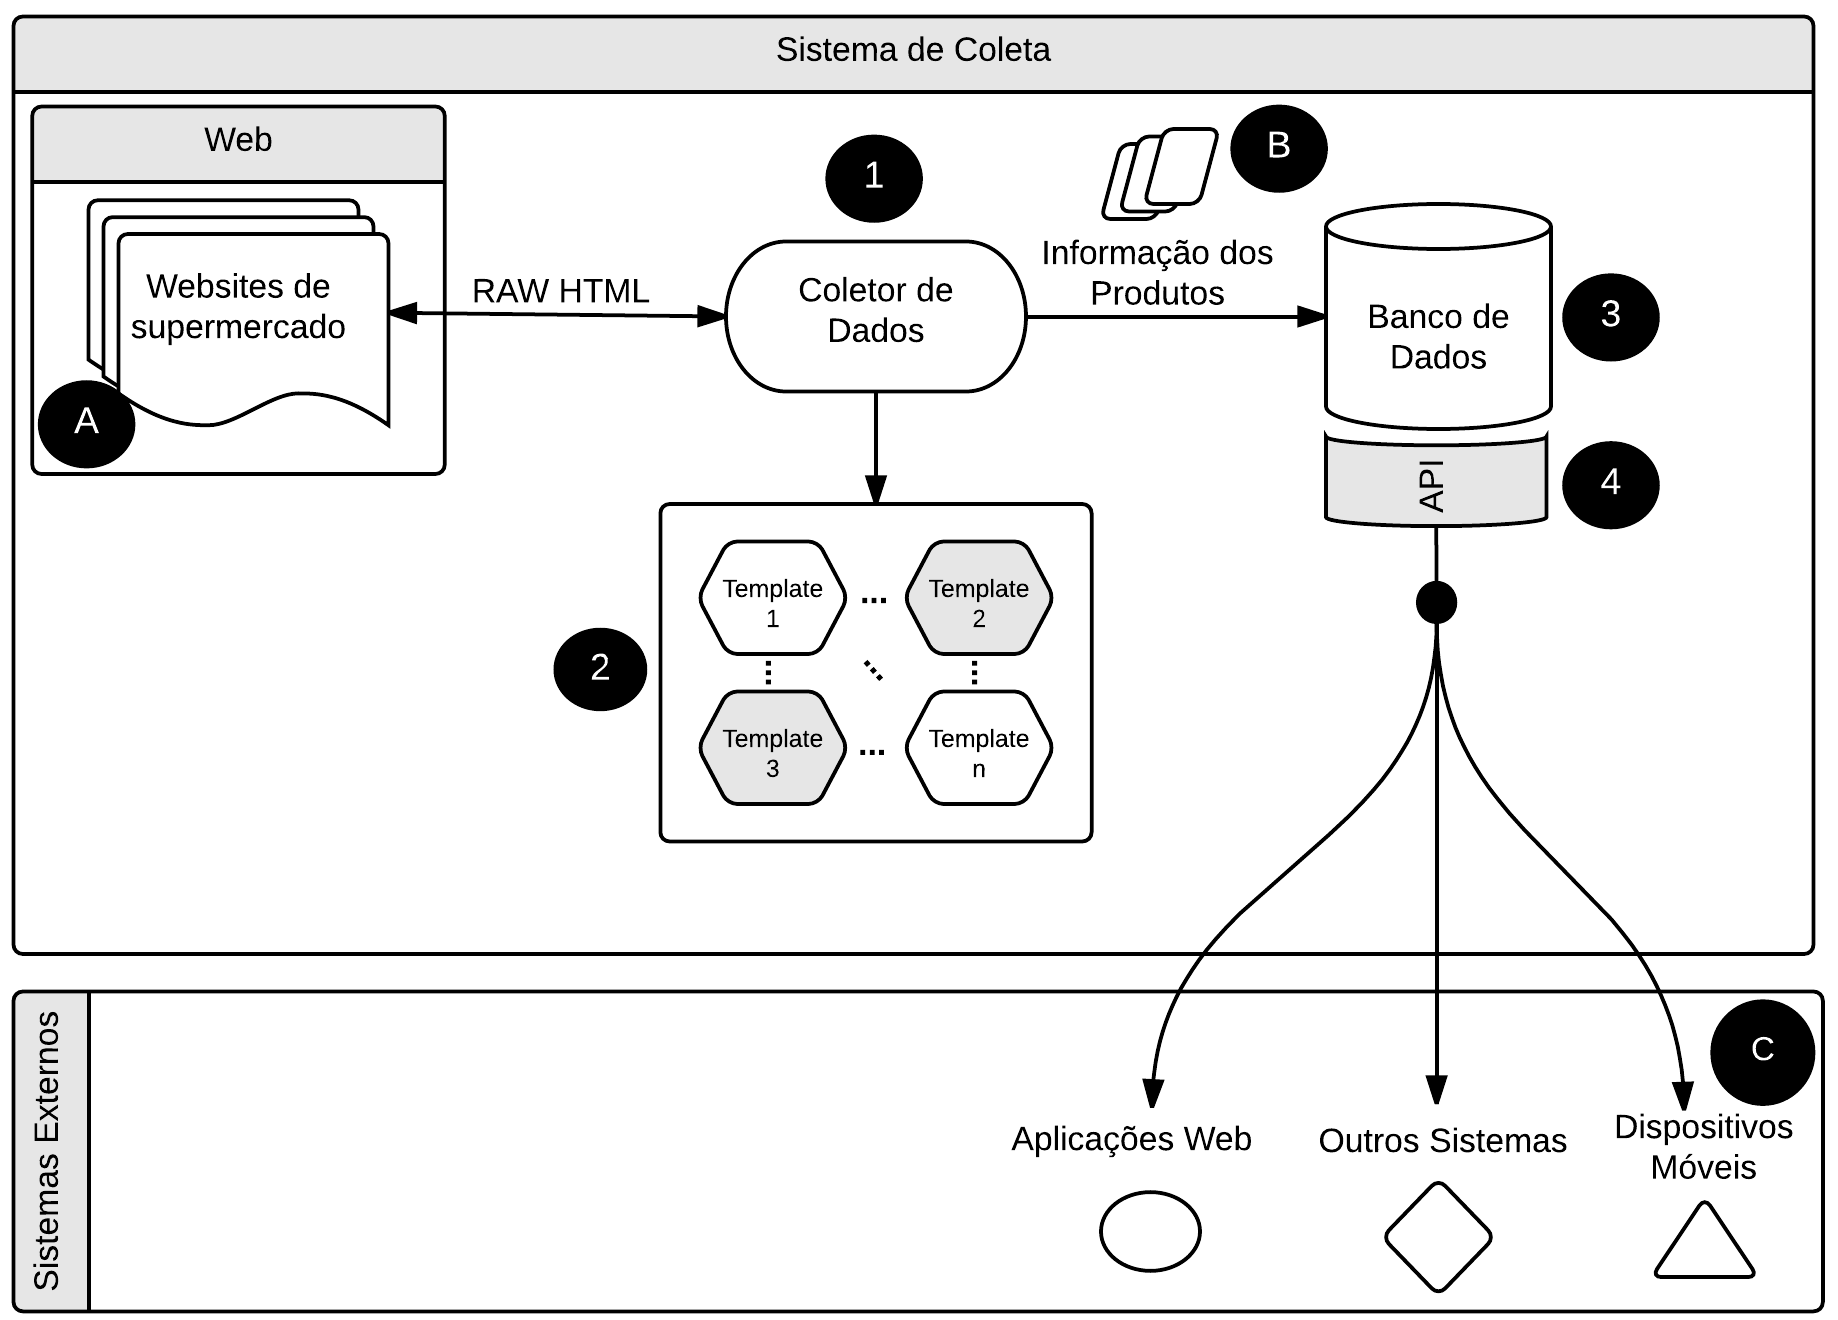
\includegraphics[width=3in]{WebScraping.png}
  \label{fig01en01}
  \caption{Arquitetura do Sistema de Coleta e Disponibilização dos Dados}
  \end{figure}
\end{frame}

\begin{frame}
\begin{centering}
\scalebox{0.95}{%
\begin{algorithm}[H]
 \Dados{T $\leftarrow$ (t)${^N_{i=1}}$; tal que T é uma lista de templates}
 \Resultado{Armazenados produtos estruturados em um banco NoSQL}
 \BlankLine
 \SetKwFunction{conectarNoSQL}{conectarNoSQL}
 \SetKwFunction{visitarWebsite}{visitarWebsite}
 \SetKwFunction{extrairInfo}{extrairInfo}
 \SetKwFunction{estruturarProduto}{estruturarProduto}
 \SetKwFunction{armazenarEmNoSQL}{armazenarEmNoSQL}
 \emph{Inicialização:} nosql $\leftarrow$ \conectarNoSQL{url, porta, ...}\;
 \BlankLine
 \For{(t, u) \textbf{in} T}{
   rawHtml $\leftarrow$ \visitarWebsite{u}\;
   P $\leftarrow$ \extrairInfo{rawHtml, t}\;
 	\For{p \textbf{in} P}{
 	ps $\leftarrow$ \estruturarProduto{p}\;
 	nosql.\armazenarEmNoSQL{ps}\;
 	}
 }
 \caption{Algoritmo para coleta de dados.}
\end{algorithm}}
\end{centering}
\end{frame}

% \begin{figure}[hb]
%   \centering
%   \includegraphics[width=4in]{gecko}
%   \caption[Close up of \textit{Hemidactylus} sp.]
%    {Close up of \textit{Hemidactylus} sp., which is
%    part the genus of the gecko family. It is the
%    second most speciose genus in the family.}
% \end{figure}

\end{document}


% %%%%%%% REFERÊNCIAL BIBLIOGRÁFICO
% 
% \section{REFERÊNCIAS}
% \begin{frame}{Bibliography}
% \bibliographystyle{apalike}
% \bibliography{geral}
 
\end{document}
